\documentclass[tikz,border=8pt]{standalone}
\usepackage{tikz}
\usetikzlibrary{arrows.meta,calc}

\begin{document}
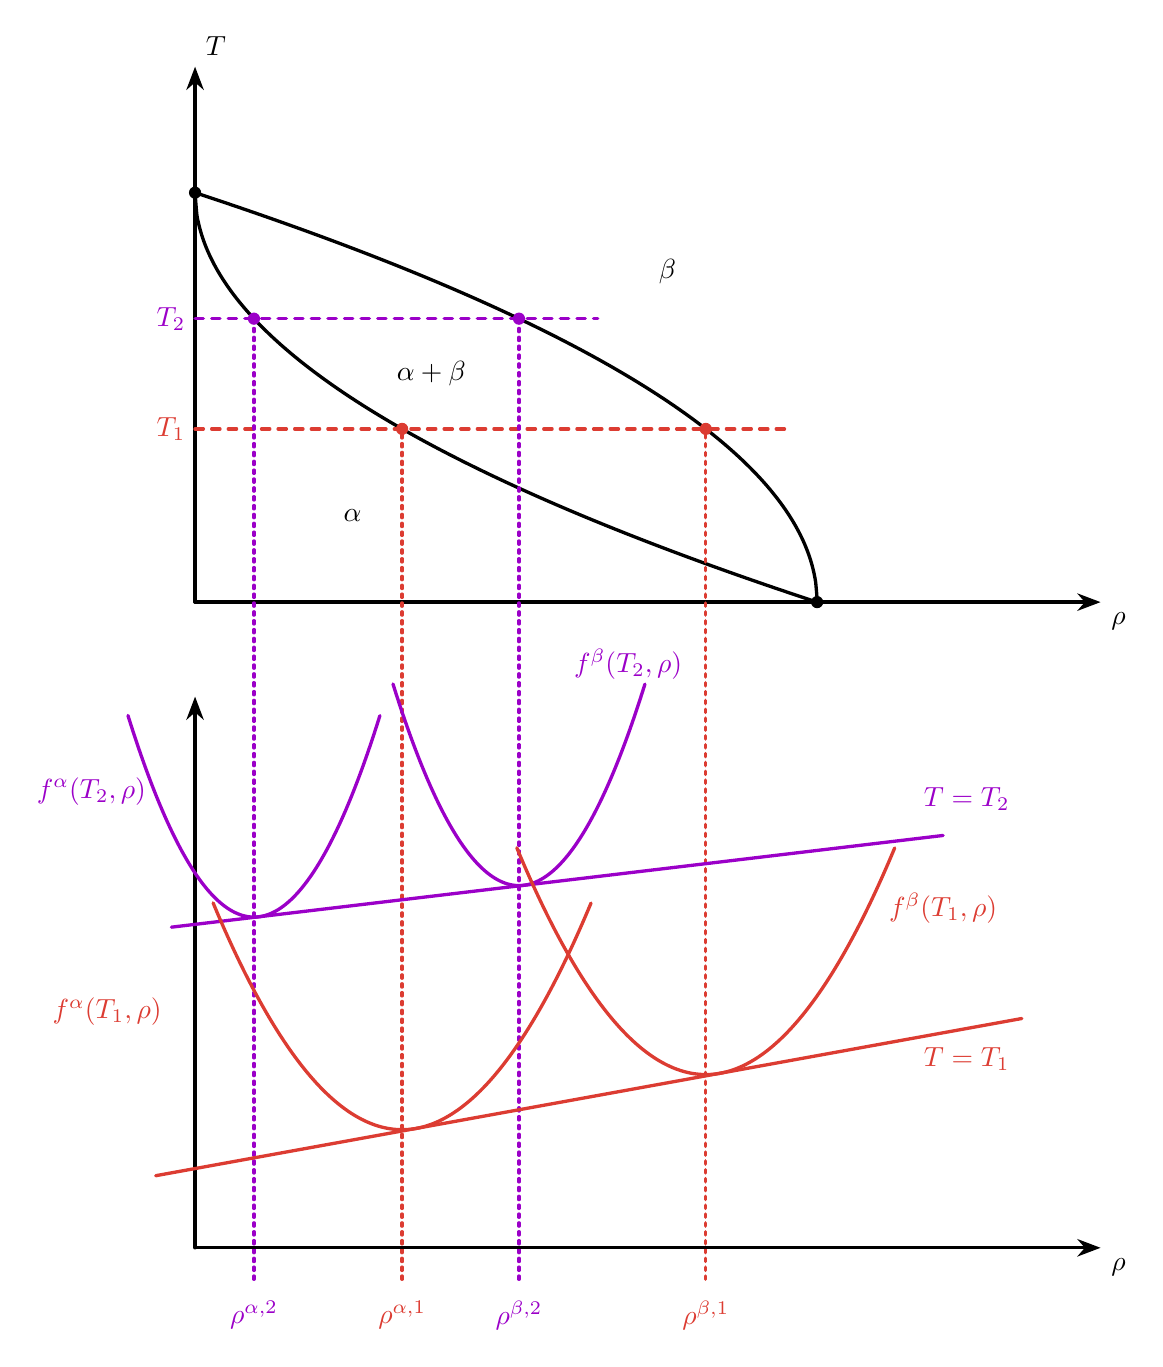
\begin{tikzpicture}[>=Stealth, line cap=round, line join=round]

% ============================================================
% KNOBS
% ============================================================
\def\W{11.5}
\def\TopH{6.0}
\def\Gap{2.0}
\def\BotH{6.2}
\def\yTop{0}
\pgfmathsetmacro{\yBot}{-(\Gap+\BotH)}

\def\TOne{2.2}
\def\TTwo{3.6}

\def\Tc{5.2}
\def\B{7.9} % BOTH top curves meet at (rho,T)=(B,0)

\definecolor{myPurple}{RGB}{155,0,200}
\definecolor{myRed}{RGB}{220,60,50}

% ============================================================
% TOP PANEL: shared x-intercept at rho=B
%   Left:  T = Tc*(1 - sqrt(rho/B))
%   Right: T = Tc*sqrt(1 - rho/B)
% ============================================================
\pgfmathsetmacro{\rhoAOne}{\B*pow(1-\TOne/\Tc,2)}
\pgfmathsetmacro{\rhoATwo}{\B*pow(1-\TTwo/\Tc,2)}
\pgfmathsetmacro{\rhoBOne}{\B*(1 - pow(\TOne/\Tc,2))}
\pgfmathsetmacro{\rhoBTwo}{\B*(1 - pow(\TTwo/\Tc,2))}

% --- TOP AXES
\draw[very thick,->] (0,\yTop) -- (0,\yTop+\TopH+0.8) node[above right] {$T$};
\draw[very thick,->] (0,\yTop) -- (\W,\yTop) node[below right] {$\rho$};

% Left boundary
\draw[very thick, samples=350, smooth, domain=0:\B]
  plot (\x, { \Tc*(1 - sqrt(\x/\B)) });

% Right boundary
\draw[very thick, samples=450, smooth, domain=0:\B]
  plot (\x, { \Tc*sqrt(1 - \x/\B) });

% Endpoints
\fill (0,\Tc) circle (2.2pt);
\fill (\B,0)  circle (2.2pt);

% Region labels
\node at (2.0,1.1) {$\alpha$};
\node at (6.0,4.2) {$\beta$};
\node at (3.0,2.9) {$\alpha+\beta$};

% Tie lines
\draw[myPurple, dashed, very thick] (0,\TTwo) -- (\rhoBTwo+1.0,\TTwo);
\node[myPurple, left] at (0,\TTwo) {$T_2$};

\draw[myRed, dashed, very thick] (0,\TOne) -- (\rhoBOne+1.0,\TOne);
\node[myRed, left] at (0,\TOne) {$T_1$};

% Points
\fill[myPurple] (\rhoATwo,\TTwo) circle (2.2pt);
\fill[myPurple] (\rhoBTwo,\TTwo) circle (2.2pt);
\fill[myRed]    (\rhoAOne,\TOne) circle (2.2pt);
\fill[myRed]    (\rhoBOne,\TOne) circle (2.2pt);

% Point labels
%\node[myPurple, above left]  at (\rhoATwo,\TTwo) {$\rho^{\alpha,2}$};
%\node[myPurple, above right] at (\rhoBTwo,\TTwo) {$\rho^{\beta,2}$};
%\node[myRed, below right]    at (\rhoAOne,\TOne) {$\rho^{\alpha,1}$};
%\node[myRed, above right]    at (\rhoBOne,\TOne) {$\rho^{\beta,1}$};

% Vertical dotted guides (spanning both panels)
\draw[myPurple, dotted, very thick] (\rhoATwo,\yBot-0.4) -- (\rhoATwo,\TTwo);
\draw[myPurple, dotted, very thick] (\rhoBTwo,\yBot-0.4) -- (\rhoBTwo,\TTwo);
\draw[myRed, dotted, very thick]    (\rhoAOne,\yBot-0.4) -- (\rhoAOne,\TOne);
\draw[myRed, dotted, very thick]    (\rhoBOne,\yBot-0.4) -- (\rhoBOne,\TOne);

% ============================================================
% BOTTOM PANEL: Free energy curves with common tangent construction
% ============================================================

% Axes
\draw[very thick,->] (0,\yBot) -- (0,\yBot+\BotH+0.8);
\draw[very thick,->] (0,\yBot) -- (\W,\yBot) node[below right] {$\rho$};

% ============================================================
% PURPLE (T2) parabolas and tangent - higher temperature
% ============================================================
% Parabola parameters for T2
\pgfmathsetmacro{\kPurple}{1.0}        % curvature coefficient
\pgfmathsetmacro{\yMinAlphaTwo}{\yBot+4.2}  % minimum height of alpha parabola
\pgfmathsetmacro{\yMinBetaTwo}{\yBot+4.6}   % minimum height of beta parabola

% Common tangent calculation for same-curvature parabolas:
% delta = (y2 - y1) / (2*k*(c2 - c1))
% Touch points: t1 = c1 + delta, t2 = c2 + delta
% Slope: m = 2*k*delta
\pgfmathsetmacro{\deltaPurple}{(\yMinBetaTwo - \yMinAlphaTwo) / (2*\kPurple*(\rhoBTwo - \rhoATwo))}
\pgfmathsetmacro{\touchAlphaTwo}{\rhoATwo + \deltaPurple}
\pgfmathsetmacro{\touchBetaTwo}{\rhoBTwo + \deltaPurple}
\pgfmathsetmacro{\mTwo}{2*\kPurple*\deltaPurple}
% y-value at touch point on alpha parabola
\pgfmathsetmacro{\yTouchAlphaTwo}{\yMinAlphaTwo + \kPurple*\deltaPurple*\deltaPurple}
% y-intercept: b = y_touch - m * x_touch
\pgfmathsetmacro{\bTwo}{\yTouchAlphaTwo - \mTwo*\touchAlphaTwo}

% Draw purple parabolas
\pgfmathsetmacro{\hwPurple}{1.6}  % half-width of parabolas
\pgfmathsetmacro{\pAiiL}{\rhoATwo-\hwPurple}
\pgfmathsetmacro{\pAiiR}{\rhoATwo+\hwPurple}
\pgfmathsetmacro{\pBiiL}{\rhoBTwo-\hwPurple}
\pgfmathsetmacro{\pBiiR}{\rhoBTwo+\hwPurple}

\draw[myPurple, very thick, samples=100, smooth, domain=\pAiiL:\pAiiR]
  plot (\x, { \yMinAlphaTwo + \kPurple*(\x-\rhoATwo)*(\x-\rhoATwo) });

\draw[myPurple, very thick, samples=100, smooth, domain=\pBiiL:\pBiiR]
  plot (\x, { \yMinBetaTwo + \kPurple*(\x-\rhoBTwo)*(\x-\rhoBTwo) });

% Purple tangent line (extends beyond touch points)
\pgfmathsetmacro{\pTangLeftX}{-0.3}
\pgfmathsetmacro{\pTangLeftY}{\bTwo + \mTwo*(-0.3)}
\pgfmathsetmacro{\pTangRightX}{9.5}
\pgfmathsetmacro{\pTangRightY}{\bTwo + \mTwo*9.5}
\draw[myPurple, very thick] (\pTangLeftX, \pTangLeftY) -- (\pTangRightX, \pTangRightY);

% Purple labels
\node[myPurple, left] at (-0.5, \yBot+5.8) {$f^\alpha(T_2,\rho)$};
\node[myPurple, above] at (5.5, \yBot+7.1) {$f^\beta(T_2,\rho)$};

% ============================================================
% RED (T1) parabolas and tangent - lower temperature
% ============================================================
\pgfmathsetmacro{\kRed}{0.5}           % curvature coefficient (wider parabolas)
\pgfmathsetmacro{\yMinAlphaOne}{\yBot+1.5}   % minimum height of alpha parabola
\pgfmathsetmacro{\yMinBetaOne}{\yBot+2.2}    % minimum height of beta parabola

% Common tangent calculation
\pgfmathsetmacro{\deltaRed}{(\yMinBetaOne - \yMinAlphaOne) / (2*\kRed*(\rhoBOne - \rhoAOne))}
\pgfmathsetmacro{\touchAlphaOne}{\rhoAOne + \deltaRed}
\pgfmathsetmacro{\touchBetaOne}{\rhoBOne + \deltaRed}
\pgfmathsetmacro{\mOne}{2*\kRed*\deltaRed}
\pgfmathsetmacro{\yTouchAlphaOne}{\yMinAlphaOne + \kRed*\deltaRed*\deltaRed}
\pgfmathsetmacro{\bOne}{\yTouchAlphaOne - \mOne*\touchAlphaOne}

% Draw red parabolas
\pgfmathsetmacro{\hwRed}{2.4}  % half-width of parabolas
\pgfmathsetmacro{\pAiL}{\rhoAOne-\hwRed}
\pgfmathsetmacro{\pAiR}{\rhoAOne+\hwRed}
\pgfmathsetmacro{\pBiL}{\rhoBOne-\hwRed}
\pgfmathsetmacro{\pBiR}{\rhoBOne+\hwRed}

\draw[myRed, very thick, samples=100, smooth, domain=\pAiL:\pAiR]
  plot (\x, { \yMinAlphaOne + \kRed*(\x-\rhoAOne)*(\x-\rhoAOne) });

\draw[myRed, very thick, samples=100, smooth, domain=\pBiL:\pBiR]
  plot (\x, { \yMinBetaOne + \kRed*(\x-\rhoBOne)*(\x-\rhoBOne) });

% Red tangent line
\pgfmathsetmacro{\rTangLeftX}{-0.5}
\pgfmathsetmacro{\rTangLeftY}{\bOne + \mOne*(-0.5)}
\pgfmathsetmacro{\rTangRightX}{10.5}
\pgfmathsetmacro{\rTangRightY}{\bOne + \mOne*10.5}
\draw[myRed, very thick] (\rTangLeftX, \rTangLeftY) -- (\rTangRightX, \rTangRightY);

% Red labels
\node[myRed, left] at (-0.3, \yBot+3.0) {$f^\alpha(T_1,\rho)$};
\node[myRed, above] at (9.5, \yBot+4) {$f^\beta(T_1,\rho)$};
\node[myRed] at (9.8, \yBot+2.4) {$T=T_1$};
\node[myPurple] at (9.8, \yBot+5.7) {$T=T_2$};

% Bottom rho labels
\node[myPurple, below] at (\rhoATwo,\yBot-0.55) {$\rho^{\alpha,2}$};
\node[myRed,    below] at (\rhoAOne,\yBot-0.55) {$\rho^{\alpha,1}$};
\node[myPurple, below] at (\rhoBTwo,\yBot-0.55) {$\rho^{\beta,2}$};
\node[myRed,    below] at (\rhoBOne,\yBot-0.55) {$\rho^{\beta,1}$};

\end{tikzpicture}
\end{document}